\section{Macroscopic traffic trends}
\label{section:malawi:macro}

\begin{figure}
  \centering
  \begin{subfigure}[b]{1.0\linewidth}
  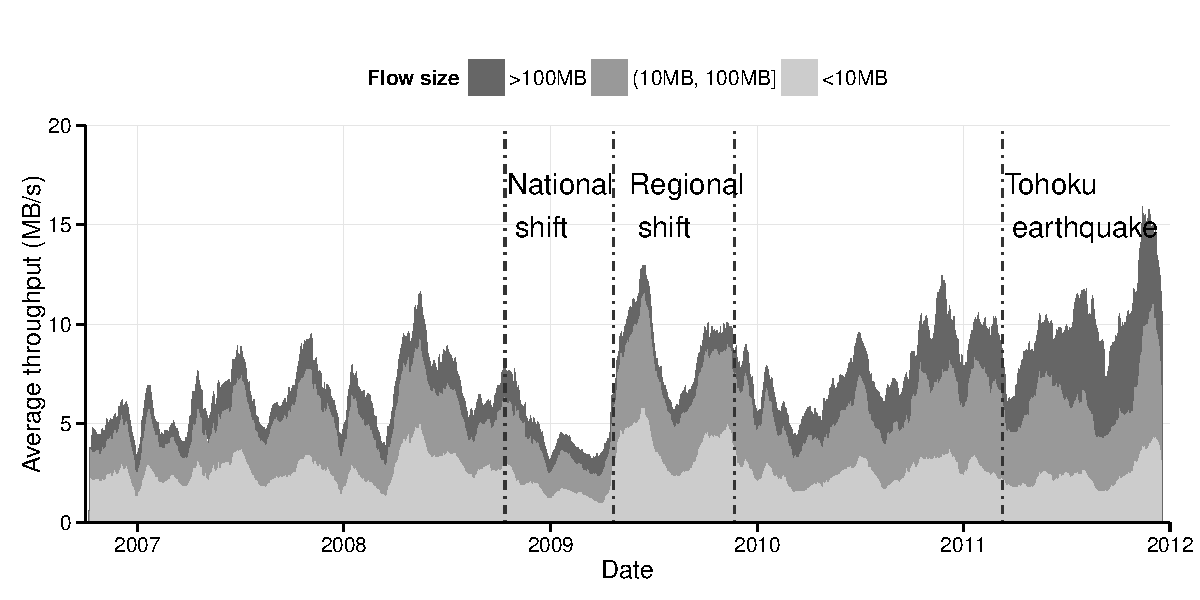
\includegraphics[width=0.9\textwidth]{figures/malawi/tput}
  \caption{Mean throughput}
  \end{subfigure}
  \begin{subfigure}[b]{1.0\linewidth}
  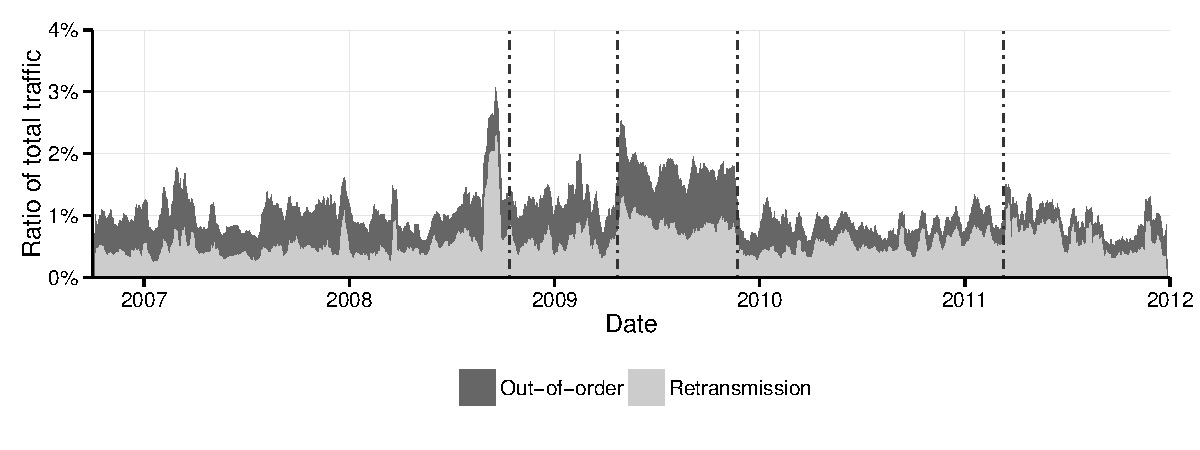
\includegraphics[width=0.9\textwidth]{figures/malawi/losses}
  \caption{Mean loss rate}
  \end{subfigure}
  \caption{Longitudinal evolution of inbound traffic.}\label{fig:MAWI}
\end{figure}

Over a five year period, changes in routing and application popularity have continually redefined the nature of traffic under observation.
In this section we provide a macroscopic view of these shifting trends. Figure \ref{fig:MAWI} displays the average throughput and loss ratio, calculated for TCP traffic only, smoothed on a weekly basis. 
Two routing changes internal to WIDE had significant impact on overall traffic, and are consequently highlighted.
The first, performed towards the end of 2008, diverted most of the inbound traffic from \emph{national} sources away from the monitored transit link, resulting in a reduction of traffic.
This event was preceded by increased congestion downstream from the monitoring point.
The second, in early 2009, saw a significant increase in \emph{regional} traffic from Asian neighbours, and was reverted approximately six months later. 
During this period aggregate end-to-end loss rates increased as a result.
While this is mostly due to the higher proportion of upstream congestion for traffic from Taiwan and China in particular, most traffic was adversely affected by the increased utilisation, suggesting that the transit link itself may have been a bottleneck during this period.
Finally, the impact of the Tohuku earthquake resulted in a noticeable break in demand coinciding with the start of the Japanese fiscal year in April, in which traffic traditionally ramps up.

\subsection{Geographic distribution}

\begin{table}\footnotesize
\centering
    \begin{tabular}{  
@{}
$>{\scshape}p{3.0cm}
^r
^r
^r
^r
^r@{\hskip 1.0cm}
^r
^r
^r
^r
^r
@{}
}
\toprule
\rowstyle{\scshape\bfseries}
\multirow{2}{*}{\parbox[][0.7cm][b]{3.0cm}{Country}} & 
\multicolumn{5}{c}{\scshape\bfseries{Outbound traffic (\%)\hspace*{0.45cm}}} & 
\multicolumn{5}{c}{\scshape\bfseries{Inbound traffic (\%)}} \\
\cmidrule(r{1.0cm}){2-6} \cmidrule{7-11}
\addlinespace[-0.6em] \rowstyle{\scriptsize\scshape}
 & 2007 & 2008 & 2009 & 2010 & 2011 & 2007 & 2008 & 2009 & 2010 & 2011 \\
\midrule

        United States & 27.3 & 31.3 & 29.3 & 36.4 & 35.7 & 45.7 & 41.5 & 53.3 & 65.1 & 67.1
\\
        \scriptsize{ California } & \scriptsize{ 39.0 } & \scriptsize{ 61.8 } & \scriptsize{ 63.5 } & \scriptsize{ 53.8 } & \scriptsize{ 50.6 } & \scriptsize{ 55.7 } & \scriptsize{ 47.9 } & \scriptsize{ 46.7 } & \scriptsize{ 24.9 } & \scriptsize{ 34.9 }\\\scriptsize{ Texas } & \scriptsize{  5.8 } & \scriptsize{  4.3 } & \scriptsize{  4.1 } & \scriptsize{  2.4 } & \scriptsize{ 13.9 } & \scriptsize{  7.0 } & \scriptsize{ 12.0 } & \scriptsize{  5.8 } & \scriptsize{  7.1 } & \scriptsize{  5.6 }\\\scriptsize{ Colorado } & \scriptsize{  1.9 } & \scriptsize{  1.2 } & \scriptsize{  0.6 } & \scriptsize{  8.5 } & \scriptsize{  2.8 } & \scriptsize{  4.9 } & \scriptsize{  6.0 } & \scriptsize{  5.9 } & \scriptsize{  9.7 } & \scriptsize{  5.8 }\\\scriptsize{ Virginia } & \scriptsize{  1.9 } & \scriptsize{  1.0 } & \scriptsize{  0.8 } & \scriptsize{  0.4 } & \scriptsize{  0.6 } & \scriptsize{  1.2 } & \scriptsize{  3.0 } & \scriptsize{ 14.1 } & \scriptsize{ 13.1 } & \scriptsize{  8.3 }\\\scriptsize{ Washington } & \scriptsize{  4.0 } & \scriptsize{  2.9 } & \scriptsize{  3.5 } & \scriptsize{  6.1 } & \scriptsize{  6.6 } & \scriptsize{  0.9 } & \scriptsize{  5.7 } & \scriptsize{  3.5 } & \scriptsize{  3.0 } & \scriptsize{  2.0 }\\\scriptsize{ New Jersey } & \scriptsize{  2.8 } & \scriptsize{  1.5 } & \scriptsize{  0.7 } & \scriptsize{  1.1 } & \scriptsize{  1.9 } & \scriptsize{  1.0 } & \scriptsize{  1.8 } & \scriptsize{  1.6 } & \scriptsize{  4.9 } & \scriptsize{ 13.6 }\\\scriptsize{ Massachusetts } & \scriptsize{  1.6 } & \scriptsize{  1.1 } & \scriptsize{  0.9 } & \scriptsize{  6.1 } & \scriptsize{  4.9 } & \scriptsize{  5.4 } & \scriptsize{  2.1 } & \scriptsize{  1.8 } & \scriptsize{  1.6 } & \scriptsize{  2.0 }\\\scriptsize{ Florida } & \scriptsize{  3.1 } & \scriptsize{  2.3 } & \scriptsize{  1.3 } & \scriptsize{  1.1 } & \scriptsize{  0.9 } & \scriptsize{  1.0 } & \scriptsize{  0.4 } & \scriptsize{  0.4 } & \scriptsize{  8.5 } & \scriptsize{  7.9 }
\\
        Japan & 11.6 & 15.4 & 17.7 & 16.7 & 16.1 & 33.8 & 32.2 &  7.3 & 8.1 & 11.5\\China &  7.9 & 20.5 & 17.8 & 10.3 &  5.9 &  2.5 &  5.3 &  6.3 & 4.6 &  3.1\\Korea, Republic of &  5.3 &  1.3 &  2.1 &  7.8 & 23.8 &  4.7 &  5.1 &  3.2 & 1.1 &  0.5\\Germany &  2.2 &  1.7 &  1.6 &  1.0 &  0.6 &  3.0 &  6.1 &  5.3 & 5.5 &  1.4\\Taiwan &  2.7 &  1.3 &  4.0 &  3.6 &  2.7 &  0.8 &  0.9 & 10.9 & 0.9 &  0.4\\Netherlands &  0.4 &  0.4 &  0.5 &  0.3 &  0.4 &  0.9 &  1.0 &  4.1 & 6.2 &  6.9\\India &  2.8 &  3.3 &  4.8 &  3.3 &  2.0 &  0.3 &  0.1 &  0.0 & 0.2 &  0.0\\France &  1.2 &  1.1 &  0.9 &  0.9 &  0.9 &  1.6 &  1.2 &  2.6 & 3.4 &  1.7\\United Kingdom &  1.1 &  1.0 &  1.0 &  0.9 &  0.7 &  2.5 &  2.2 &  1.6 & 1.3 &  1.3
\\
    \end{tabular}
  \caption{Percentage of inbound and outbound traffic by country\label{table:dest}. U.S. state values are relative to total national traffic.}
\end{table}



These changes are both visible in the geographic distribution of inbound traffic over time, shown in table \ref{table:dest}.
Prior to 2009, a significant proportion of transit traffic originated from within Japan. Over time, however, the ratio of traffic from Asia has been reduced. While this may foreshadow an increased concentration of traffic from the United States, it should primarily be viewed as a reflection of routing policy, with regional traffic being diverted to alternate routes as Japan became increasingly interconnected to its neighbours.


Further geographic shifts are apparent when breaking down US traffic by state.
The proportion of traffic originating from California has decreased over time, dropping from 55\% of total US traffic in 2007 to only 35\% in 2011.
In its place, a larger set of states have emerged as content providers, with New Jersey, Florida and Virginia contributing over a quarter of all traffic originating within the US by 2011.

\subsection{\acs{AS}-level distribution}

\begin{figure}
    \centering
    \begin{subfigure}[b]{0.5\linewidth}
        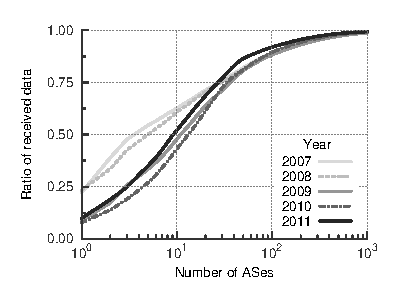
\includegraphics{figures/malawi/asn_cdf_in}
        \caption{Inbound}
    \end{subfigure}%
    \begin{subfigure}[b]{0.5\linewidth}
        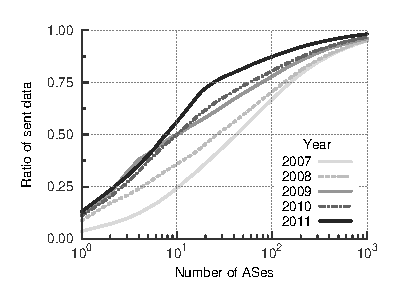
\includegraphics{figures/malawi/asn_cdf_out}
        \caption{Outbound}
    \end{subfigure}%
    \caption{CDF of inbound data by AS. \label{fig:ecdf_asn_from}}
\end{figure}


%\begin{table*}\scriptsize
%\centering
%\subfloat[2007]{
    %\begin{tabular}{
@{}
$>{\raggedleft}p{0.6cm}
^>{\scshape}p{2.25cm}
^>{\raggedleft\arraybackslash}p{0.6cm}
@{}
}
\toprule
\rowstyle{\scshape\bfseries}
\acs{ASN} & \acs{AS} name &
\% \\
\midrule

    %\input{data/malawi/asn2007.tex}
    %\end{tabular} % closes asnheader.tex tabular environment
    %}
%\subfloat[2009]{
    %\begin{tabular}{
@{}
$>{\raggedleft}p{0.6cm}
^>{\scshape}p{2.25cm}
^>{\raggedleft\arraybackslash}p{0.6cm}
@{}
}
\toprule
\rowstyle{\scshape\bfseries}
\acs{ASN} & \acs{AS} name &
\% \\
\midrule

    %\input{data/malawi/asn2009.tex}
    %\end{tabular} % closes asnheader.tex tabular environment
%}
%\subfloat[2011]{
    %\begin{tabular}{
@{}
$>{\raggedleft}p{0.6cm}
^>{\scshape}p{2.25cm}
^>{\raggedleft\arraybackslash}p{0.6cm}
@{}
}
\toprule
\rowstyle{\scshape\bfseries}
\acs{ASN} & \acs{AS} name &
\% \\
\midrule

    %\input{data/malawi/asn2011.tex}
    %\end{tabular} % closes asnheader.tex tabular environment
%}
%\caption{
    %\label{table:topASin}
    %Top 10 ASes for inbound traffic by year. Additionally listed is the ratio of aggregate end-to-end loss.}
%\vspace{-3mm}
%\end{table*}


These large-scale changes are a natural outcome of content consolidation. This is most apparent at the AS level, where a direct mapping to a commercial entity is forthcoming.
Figure \ref{fig:ecdf_asn_from} shows the cumulative distribution of inbound traffic by AS, while table \ref{table:topASin} lists the top ten AS by traffic volume for 2007, 2009 and 2011.
While in 2007 traffic was already consolidated across a small set of ASes, a significant portion of transit traffic was Asian: most traffic from NTT and Limelight originated from within Japan. Such traffic has gradually been pushed away from transit by 2011.
Large carriers such as Cogent, Level3, Hanaro, China Telecom have also seen their importance diluted by ASes known to harbour one-click hosting services such as Choopa, Webazilla, WZ Communications, Carpathia and LeaseWeb.
Many of the hosted websites facilitate the distribution of copyrighted content, and as such are not capable of growing large enough to expand beyond hosted infrastructure without risking prosecution.
% overall summary: content consolidation, delay, etc
Overall, the observed traffic patterns match the insights provided by Labovitz et al. on the changing nature of interdomain traffic in \cite{Labovitz:2010p175}.
The implications for transit traffic from an Asian perspective is less intuitive: with the increased adoption of content delivery networks and internet exchanges points, more transit traffic is being retrieved from further away as content in the US shifts east.

\subsection{Delay}


\begin{figure}
    \centering
    \begin{subfigure}[b]{0.5\linewidth}
        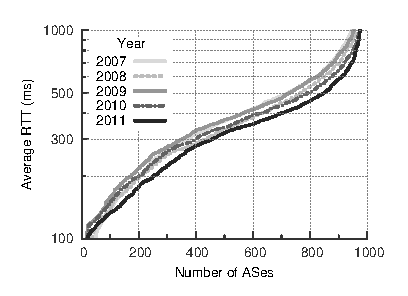
\includegraphics{figures/malawi/rtt_cdf_in}
        \caption{Inbound}
    \end{subfigure}%
    \begin{subfigure}[b]{0.5\linewidth}
        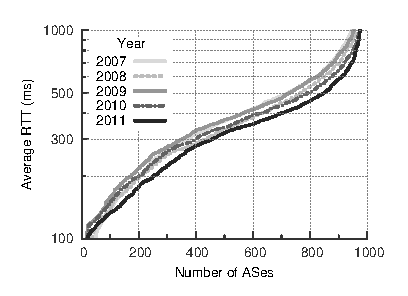
\includegraphics{figures/malawi/rtt_cdf_out}
        \caption{Outbound}
    \end{subfigure}%
    \caption{CDF of RTT by AS. \label{fig:rtt_cdf}}
\end{figure}

\begin{figure}
    \centering
    \begin{subfigure}[b]{0.5\linewidth}
        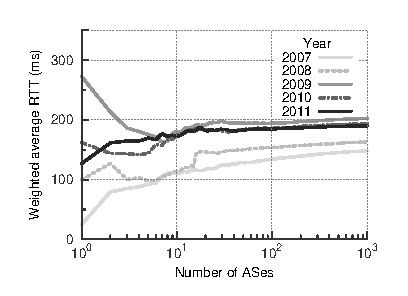
\includegraphics{figures/malawi/rtt_wcdf_in}
        \caption{Inbound}
    \end{subfigure}%
    \begin{subfigure}[b]{0.5\linewidth}
        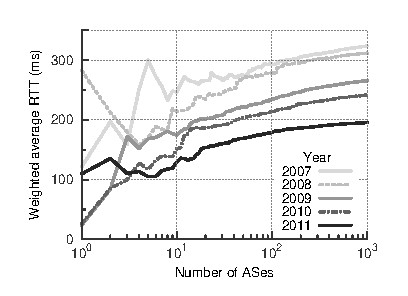
\includegraphics{figures/malawi/rtt_wcdf_out}
        \caption{Outbound}
    \end{subfigure}%
    \caption{CDF of weighted RTT by AS. \label{fig:rtt_wcdf}}
\end{figure}

\begin{figure}
    \centering
    \begin{subfigure}[b]{0.5\linewidth}
        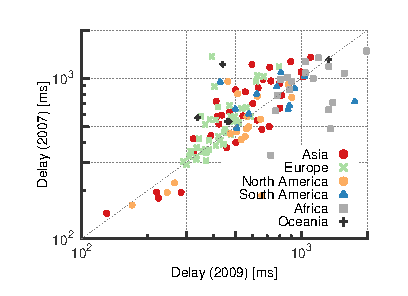
\includegraphics{figures/malawi/rtt_comp_07_09}
        \caption{Inbound}
    \end{subfigure}%
    \begin{subfigure}[b]{0.5\linewidth}
        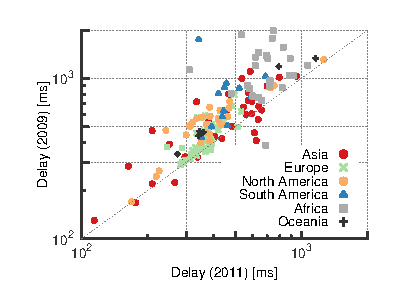
\includegraphics{figures/malawi/rtt_comp_09_11}
        \caption{Outbound}
    \end{subfigure}%
    \caption{CDF of weighted RTT by AS. \label{fig:rtt_comp}}
\end{figure}

